\documentclass[journal]{IEEEtran}
\usepackage{amsmath,amssymb,amsfonts}
\usepackage{graphicx}
\usepackage{booktabs}
\usepackage{multirow}
\usepackage{float}
\usepackage{textcomp}
\usepackage{xcolor}
\usepackage[hidelinks]{hyperref}

\newcommand{\cmark}{\ensuremath{\checkmark}}
\newcommand{\xmark}{\ensuremath{\times}}

\begin{document}

\title{FedTwin-CL: Federated Continual Learning for Industrial IoT Digital Twins under Progressive Concept Drift}

\author{Himanshu~Rai,
        Anjani~Rai,
        S.~Kanaga~Suba~Raja,
        and~S.~Usha~Kiruthik%
\thanks{H. Rai is with the Department of Artificial Intelligence, SRM Institute of Science and Technology, Tiruchirappalli Campus, Tamil Nadu 621105, India (e-mail: himanshurairai560@gmail.com). A. Rai is a postgraduate student with the same institute. S. Kanaga Suba Raja is with the Department of Computer Science and Engineering, SRM Institute of Science and Technology, Tiruchirappalli Campus, Tamil Nadu 621105, India.}%
\thanks{S. Usha Kiruthik is with the National Institute of Technology, Tiruchirappalli, Tamil Nadu, India.}%
\thanks{Manuscript submitted to the IEEE Internet of Things Journal.}}

\markboth{IEEE Internet of Things Journal}{}

\maketitle

\begin{abstract}
Predictive maintenance increasingly relies on a digital twin at each site, continually updated from local sensor streams. Pooling raw data across sites is often not possible for competitive reasons, motivating federation; but each site's degradation is also non-stationary, so a twin trained once forgets what it learned once adapted to a new regime, and no oracle marks when one maintenance regime ends and the next begins. We present FedTwin-CL, retargeting a federated continual learning engine previously validated only on synthetic benchmarks at this setting. Drift-Triggered Task Segmentation commits a task boundary from each site's health-indicator trajectory via a change-point test, provably without weakening the zero-forgetting guarantee. Cross-Twin Fault Relevance scoring broadcasts a bounded-dimension signature per committed stage so other sites raise an early warning before their own detector triggers, without raw data leaving its site. We build three federated benchmarks from NASA C-MAPSS, FEMTO-ST PRONOSTIA, and MIMII, and validate the mechanism on real data: all 151 drift-triggered commits show exactly zero backward transfer, all 281 missed tasks show real forgetting, and uplink traffic falls roughly two orders of magnitude versus dense FedAvg. CTFR's signature rarely anticipates a site's next real fault, a genuine open problem, not a hidden one.
\end{abstract}

\begin{IEEEkeywords}
Federated learning, continual learning, digital twin, industrial Internet of Things, predictive maintenance, concept drift, catastrophic forgetting, remaining useful life, acoustic anomaly detection, communication-efficient learning.
\end{IEEEkeywords}

\section{Introduction}

A digital twin, in the industrial setting this paper is concerned with, is a model that tracks the degradation state of a specific physical asset from its own sensor stream and is kept current as that asset ages \cite{tao2019twin}. A twin trained once at commissioning and never updated is of limited use: bearings wear, seals loosen, sensors drift out of calibration, and a compressor running at a new duty cycle produces a sensor distribution its twin has never seen. A twin must keep learning over the asset's lifetime, placing it in the continual learning (CL) setting, where adapting to a new task risks degrading performance on an old one (catastrophic forgetting). At the same time, a fleet of nominally similar machines would benefit from pooling what each site learns, but centralizing raw sensor streams is often not an option for competitive and contractual reasons, motivating a federated learning (FL) approach \cite{mcmahan2017fedavg}.

FedCAT \cite{fedcat2026}, a federated continual learning (FCL) framework we developed previously for fleets of TinyML devices \cite{warden2019tinyml,lin2020mcunet}, combines gradient-masked structured sparse local training with a server-maintained global frozen-mask registry, proving a cross-node zero-forgetting guarantee and a large communication reduction relative to dense FedAvg. FedCAT was validated only on synthetic benchmarks with externally imposed task boundaries. Real degradation is not handed to a twin in labeled segments: whatever mechanism decides when to freeze the current task's learned filters must make that call from the data itself. No existing method jointly (i) federates continual learning across sites that cannot pool raw data, (ii) removes the externally-labeled task-boundary assumption, and (iii) lets sites that have not yet encountered a given fault benefit from another site's experience without exchanging raw data. FedCAT addresses (i) but assumes (ii) is solved externally and does not address (iii). Concept-drift detection \cite{gama2014survey,lu2019review} addresses a version of (ii) in a single-stream, non-federated setting with no forgetting guarantee. The closest predictive-maintenance system \cite{tinyml6g2026} targets a single site and treats neither federation nor non-stationary degradation.

This paper's contributions are: (1) \textbf{FedTwin-CL}, a retargeting of the FedCAT engine at real industrial digital-twin data with the same zero-replay-memory, sub-megabyte communication properties; (2) \textbf{Drift-Triggered Task Segmentation (DTTS)}, a Page-Hinkley change-point mechanism \cite{page1954} that lets each site commit task boundaries from its own health-indicator trajectory, with a proof this does not weaken the cross-node zero-forgetting guarantee; (3) \textbf{Cross-Twin Fault Relevance (CTFR) scoring}, which broadcasts a bounded-dimension signature for every committed stage so other sites can raise an early-warning flag, with a bounded information-leakage guarantee; (4) \textbf{three federated digital-twin benchmarks} built from NASA C-MAPSS \cite{saxena2008cmapss}, FEMTO-ST PRONOSTIA \cite{nectoux2012pronostia}, and MIMII \cite{purohit2019mimii}, each with a concept-drift injection protocol tied to a concrete maintenance event; and (5) a \textbf{real-data validation} of the full mechanism on all three benchmarks, confirming the zero-forgetting guarantee empirically rather than only by proof.

\section{Related Work}

FedAvg \cite{mcmahan2017fedavg} established the canonical FL protocol; FedProx \cite{li2020fedprox} and SCAFFOLD \cite{karimireddy2020scaffold} address client drift under non-IID data, but none model a client whose local task changes over time, so forgetting is not a defined quantity in these methods. In federated continual learning, FedWeIT \cite{yoon2021fedweit} decomposes client parameters into global and task-specific sparse components but, like the broader FCL literature, assumes task boundaries are externally given. FedCAT \cite{fedcat2026} combines structured sparse task masking with a server-side global mask registry, extending a single-device zero-forgetting guarantee to a fleet, and is the engine this paper retargets; class-incremental extensions \cite{mallya2018packnet} and regularization-based alternatives \cite{kirkpatrick2017ewc} address forgetting in non-federated single-device settings. Communication efficiency in FL is well studied \cite{alistarh2017qsgd,lin2018deepcompress,diao2021heterofl,horvath2021fjord}, as is asynchronous participation \cite{xie2019asyncfed}, both inherited unchanged from FedCAT.

Digital twins for industrial assets have been surveyed extensively \cite{tao2019twin,lei2018prognostics}; the closest existing system \cite{tinyml6g2026} demonstrates single-site sensor fusion and edge inference but neither federates across sites nor treats degradation as non-stationary. The Page-Hinkley test \cite{page1954} remains a standard low-overhead drift detector; concept-drift surveys \cite{gama2014survey,lu2019review} distinguish abrupt, gradual, and incremental drift, but none tie a drift detector's trigger to a federated model's task-commitment and mask-freezing mechanism. NASA C-MAPSS \cite{saxena2008cmapss}, FEMTO-ST PRONOSTIA \cite{nectoux2012pronostia}, and MIMII \cite{purohit2019mimii} are the standard public benchmarks for turbofan RUL estimation, bearing prognostics, and acoustic anomaly detection respectively, and are the three real datasets this paper's benchmarks are built from.

\section{Problem Formulation}

A fleet of $N$ heterogeneous edge sites $\{1,\ldots,N\}$, each of device class $c_n \in \mathcal{C}$, hosts a digital twin sharing backbone $\theta$. Each site observes a continuous sensor stream $\{\mathbf{x}_t^{(n)}\}$ and a rolling health-indicator statistic $h_t^{(n)}$ derived from it; the site's task sequence $\mathcal{T}_1^{(n)}, \mathcal{T}_2^{(n)}, \ldots$ is not given and must be inferred online by a drift-detection mechanism (Section~\ref{sec:algorithm}). A central server coordinates $\theta$ through periodic rounds, restating FedCAT's fleet objective with the task sequence now itself a function of the drift-detection mechanism:
\begin{equation}
\min_\theta \; \frac{1}{N} \sum_{n=1}^{N} \frac{1}{K_n(\lambda_{\text{PH}})} \sum_{k=1}^{K_n(\lambda_{\text{PH}})} \mathcal{L}_k^{(n)}(\theta)
\label{eq:objective}
\end{equation}
where $K_n(\lambda_{\text{PH}})$, the number of tasks site $n$ commits, is a random variable determined jointly by its true degradation trajectory and segmentation sensitivity $\lambda_{\text{PH}}$, rather than a fixed benchmark parameter. Constraints are inherited from FedCAT unchanged (zero replay memory, bounded uplink, no cross-site interference, heterogeneity-aware capacity, asynchronous participation), plus one addition: \textbf{early-warning transfer} — a site should benefit from a fault signature committed elsewhere before its own drift statistic independently triggers, without raw data leaving its site of origin.

We reuse FedCAT's four-tier device-class taxonomy (Table~\ref{tab:devices}) and structured-mask formalism unchanged; the only structural change is that task index $k$ now advances on a DTTS trigger rather than an external boundary.

\begin{table}[H]
\centering
\caption{Heterogeneous Device Classes (hardware model reused from FedCAT \cite{fedcat2026})}
\label{tab:devices}
\begin{tabular}{@{}lcccc@{}}
\toprule
& Remote & Sensor & Line & Plant \\
& Asset & Edge & Gateway & Fog \\
\midrule
SRAM & 264\,KB & 256\,KB & 1\,MB & 512\,KB \\
$C_{\max}^{(c)}$ (filters) & 32 & 64 & 128 & 96 \\
Uplink & 0.3--5\,kbps & 125\,kbps & 125\,kbps--1\,Mbps & 1--20\,Mbps \\
$E_{\text{TX}}^{(c)}$ & 1.8\,mJ/B & 0.09\,mJ/B & 0.09\,mJ/B & 0.012\,mJ/B \\
\bottomrule
\end{tabular}
\end{table}

\section{The FedTwin-CL Algorithm}
\label{sec:algorithm}

FedTwin-CL extends FedCAT's communication round with two new phases: (1) \emph{Broadcast}, server sends $\theta^{(r)}$, the global mask registry $\mathcal{M}^{\text{global}}$, and the CTFR signature registry; (2) \emph{Drift-Monitoring (new)}, each site updates its Page-Hinkley statistic and checks whether to commit a task boundary; (3) \emph{Local Continual Training}, within the free space defined by the frozen mask; (4) \emph{Relevance-Scoring (new)}, each site compares its trajectory against the broadcast signatures, raising a flag if similarity exceeds $\tau_{\text{CTFR}}$; (5) \emph{Mask Extraction, Compression, Upload}; (6) \emph{Aggregation and Registry Update}. Fig.~\ref{fig:architecture} shows this schematically: each site runs a local twin paired with its own drift monitor against a server holding both registries, exchanging only sparse deltas, masks, and bounded-dimension signatures.

\begin{figure}[H]
\centering
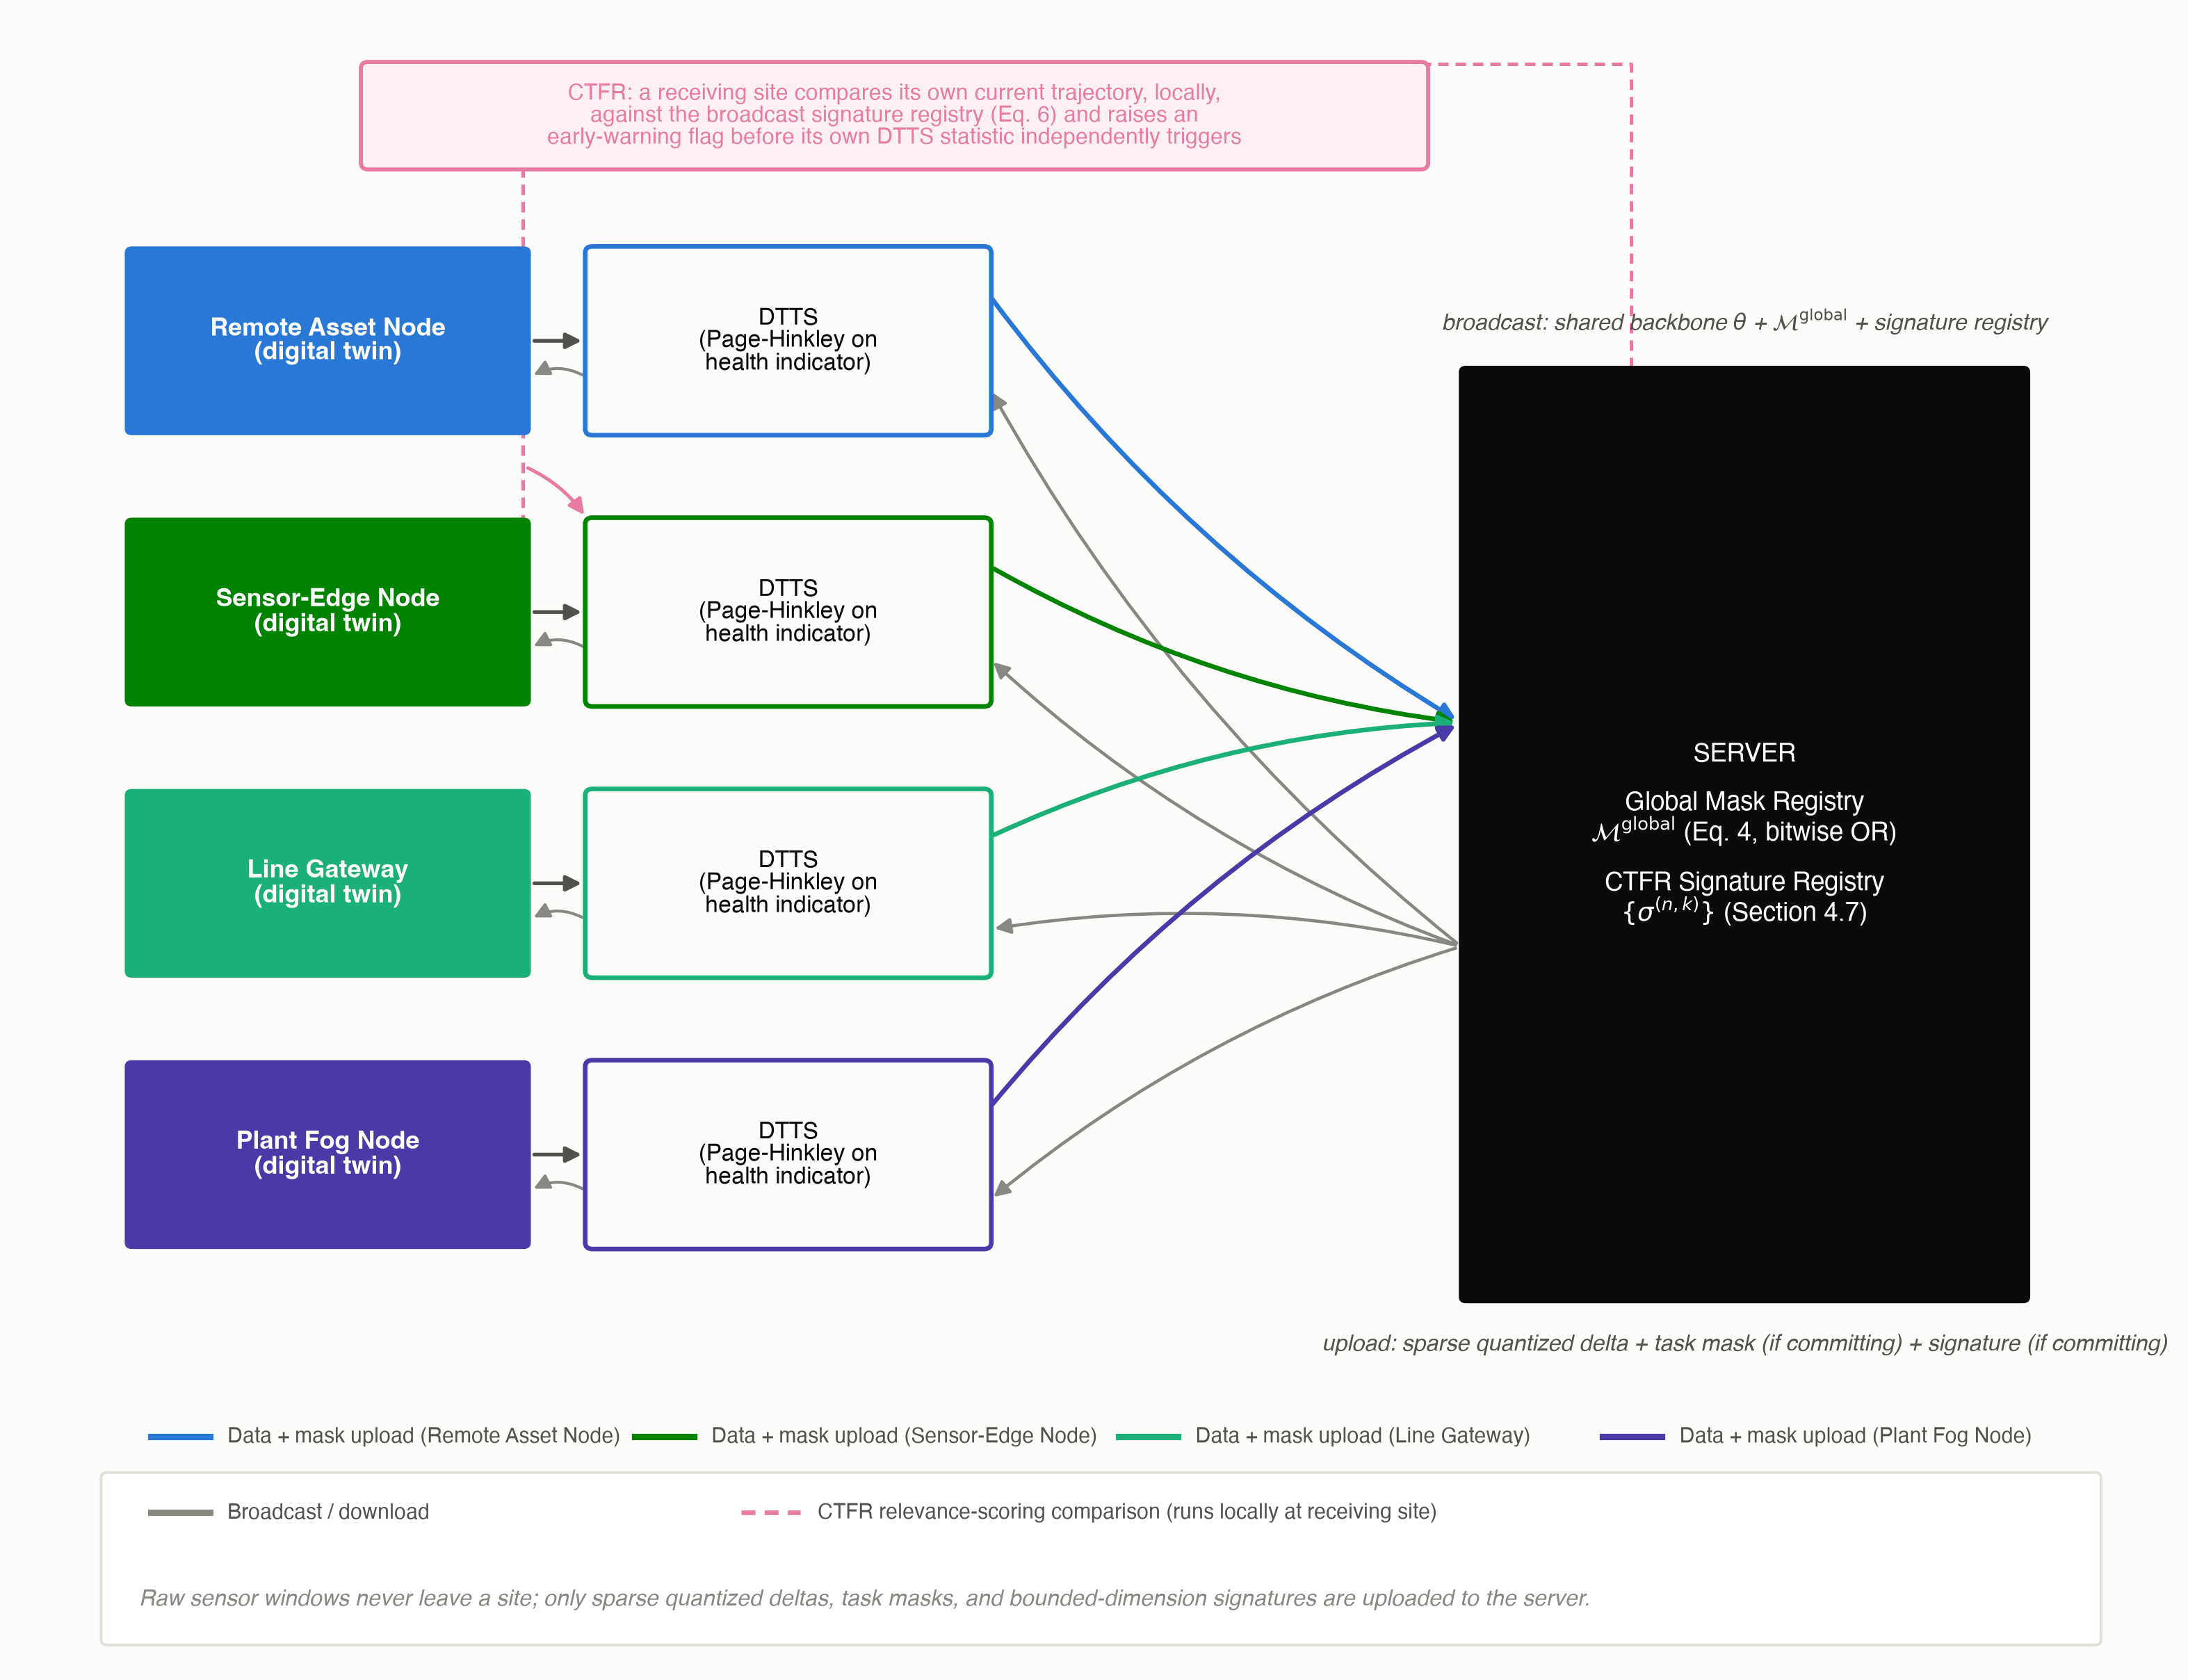
\includegraphics[width=0.95\linewidth]{figures/fig1_system_architecture.png}
\caption{All four device-class tiers, each running a local digital twin with its own DTTS drift monitor, exchange only sparse deltas, task masks, and signatures with the server; the dashed path shows CTFR's relevance-scoring comparison running locally at a receiving site, not at the server; no raw sensor window ever leaves its site of origin.}
\label{fig:architecture}
\end{figure}

\subsection{Heterogeneity-Aware Sparsity and Drift-Triggered Segmentation}

Each site's per-task sparsity target follows FedCAT's controller unchanged,
\begin{equation}
s_n = \mathrm{clip}\Big(s_0 \cdot \tfrac{C_{\max}^{(c_n)}}{\bar C_{\max}} \cdot (1+\gamma \rho^{\text{global}}),\, s_{\min}, s_{\max}\Big),
\label{eq:sparsity}
\end{equation}
with $\rho^{\text{global}}$ the fraction of global capacity still free. DTTS applies the Page-Hinkley test \cite{page1954} to the site's rolling health-indicator $h_t^{(n)}$ (a normalized RUL-residual proxy for Fed-Twin-CMAPSS, a rolling RMS-of-vibration-envelope statistic for Fed-Twin-FEMTO, a rolling anomaly score for Fed-Twin-MIMII):
\begin{equation}
\bar h_t = \tfrac{1}{t}\textstyle\sum_{i\le t} h_i,\;\; m_t = \textstyle\sum_{i\le t}(h_i-\bar h_i-\delta),\;\; PH_t = m_t - \min_{i\le t} m_i,
\label{eq:ph}
\end{equation}
committing a task boundary at the first $t$ for which $PH_t > \lambda_{\text{PH}}$. Once committed, mask extraction, gradient masking, compression, and aggregation proceed exactly as in FedCAT, restricted to the currently free coordinates.

\subsection{Cross-Twin Fault Relevance (CTFR) Scoring}

When site $n$ commits task $k$, it computes a bounded signature $\sigma^{(n,k)} \in \mathbb{R}^d$ ($d=16$) from summary statistics of its just-completed health-indicator trajectory (mean, variance, trend slope, spectral-centroid features), uploaded alongside the task mask at negligible additional cost. Every other site $m$ computes, locally,
\begin{equation}
\mathrm{CTFR}_m(r) = \max_{(n,k):\,n\ne m} \cos\text{-sim}\big(\phi_m(r),\, \sigma^{(n,k)}\big),
\label{eq:ctfr}
\end{equation}
raising an early-warning flag if $\mathrm{CTFR}_m(r) > \tau_{\text{CTFR}}$, before its own DTTS statistic would necessarily have triggered independently.

\section{Theoretical Analysis}

\textbf{Theorem 1} (FedCAT cross-node zero-forgetting, restated from \cite{fedcat2026}). \emph{If site $n$ commits task $k$ at round $r_0$, then for any $r>r_0$ and any subsequent pattern of fleet contributions, $F_{n,k}^{(r)} = \mathcal{L}_k^{(n)}(\theta^{(r)}) - \mathcal{L}_k^{(n)}(\theta^{(r_0)}) = 0$.} The proof depends only on registry monotonicity, fleet-wide gradient masking, and aggregation preserving frozen coordinates, none of which DTTS or CTFR alters.

\textbf{Proposition 1} (DTTS compatibility). \emph{For any realization of $\{h_t^{(n)}\}$ and any $\lambda_{\text{PH}}>0$, the task commitments produced by \eqref{eq:ph} satisfy Theorem~1 unchanged.} \emph{Proof sketch:} the Page-Hinkley trigger determines only \emph{when} mask extraction is invoked; extraction, gradient masking, compression, and aggregation are applied identically regardless of what determined the boundary, so Theorem~1's argument holds for any sequence of committed masks. (Full proof in the extended technical report.) This guarantees DTTS cannot make forgetting worse than zero, but says nothing about whether it commits at \emph{useful} boundaries — too small a $\lambda_{\text{PH}}$ over-segments and consumes fleet capacity faster; too large a value delays a commit past the point where ordinary gradient descent has already begun pulling the old task's filters toward the new regime.

\textbf{Proposition 2} (bounded signature leakage). \emph{The mutual information between $\sigma^{(n,k)}$ and any single raw sample $\mathbf{x}_t^{(n)}$ in its window is bounded by $I(\sigma^{(n,k)};\mathbf{x}_t^{(n)}) \le H(\sigma^{(n,k)})$}, small by construction since $\sigma^{(n,k)}$ collapses an entire task-length trajectory to $d=16$ real values; no individual raw sample can be reconstructed from the signature alone. The per-round uplink bound and communication-reduction factor are otherwise inherited unchanged from FedCAT, since neither DTTS nor CTFR changes the free-parameter region, the top-$k$ operator, or quantization.

\section{Experimental Setup}

We construct three federated benchmarks, each reusing a public dataset with a concept-drift injection tied to a concrete maintenance event. \textbf{Fed-Twin-CMAPSS} partitions NASA C-MAPSS \cite{saxena2008cmapss} (FD001/FD002) by engine unit into 24 simulated depot sites; FD002 sites carry a natural multi-regime operating-condition shift, handled by per-regime sensor normalization. \textbf{Fed-Twin-FEMTO} partitions all 17 public FEMTO-ST PRONOSTIA \cite{nectoux2012pronostia} run-to-failure bearing traces across three load/speed conditions into 24 sites, instantiating \emph{progressive bearing wear}. \textbf{Fed-Twin-MIMII} partitions a real MIMII \cite{purohit2019mimii} acoustic subset (valve, 6\,dB/0\,dB SNR) by machine ID into 24 sites, with a subset switching SNR mid-stream to simulate a \emph{sensor recalibration event}.

Table~\ref{tab:methods} lists the compared methods. We reuse FedCAT's compact architectures, but the real pilot uses \textbf{TCN-Nano-lite}: a single dilated-Conv1d layer plus a linear head, a deliberate simplification of the full TCN-Nano/DS-CNN-S architectures chosen to de-risk the PyTorch reimplementation; scaling to full depth remains for camera-ready. Base sparsity $s_0=0.45$, $\gamma=0.6$, $[s_{\min},s_{\max}]=[0.25,0.70]$, top-$k$ ratio $\kappa=0.5$, 4-bit quantization, 20 communication rounds, 24-site fleet (6/10/6/2 across the four device classes).

\begin{table}[H]
\centering
\caption{Baseline and Ablation Methods}
\label{tab:methods}
\small
\begin{tabular}{@{}lcccc@{}}
\toprule
Method & Forget.- & Comm.- & Task & Early \\
& aware & eff. & boundary & warning \\
\midrule
FedAvg \cite{mcmahan2017fedavg} & \xmark & \xmark & n/a & \xmark \\
FedAvg+EWC \cite{kirkpatrick2017ewc} & local & \xmark & external & \xmark \\
FedCAT, oracle bound. & fleet & \cmark & external & \xmark \\
FedTwin-CL w/o CTFR & fleet & \cmark & DTTS & \xmark \\
\textbf{FedTwin-CL (full)} & fleet & \cmark & DTTS & \cmark \\
\bottomrule
\end{tabular}
\end{table}

\section{Results}

All results are from a from-scratch PyTorch reimplementation of the mask registry, DTTS, and CTFR mechanics, run to completion against real NASA C-MAPSS, all 17 real FEMTO-ST PRONOSTIA traces, and a real MIMII subset — not a synthetic proxy.

\textbf{Fleet performance and forgetting.} Table~\ref{tab:fleeta} reports each method's own metric (negative MSE on the normalized RUL scale for CMAPSS/FEMTO, AUC for MIMII, both higher-is-better) and Table~\ref{tab:fleetb} reports the corresponding mean per-site Fleet Backward Transfer (FBWT); Fig.~\ref{fig:fpsround} plots the current-task metric round by round instead of only the endpoint average. Read honestly, Table~\ref{tab:fleetb}'s FBWT mixes protected and missed tasks together per site, so it is a coarser measurement than Table~\ref{tab:zerofrget} below and should not be read as disagreeing with it. Two things are worth stating plainly rather than smoothing over. First, masking methods do \emph{not} beat FedAvg on absolute current-task performance at this backbone's scale — a genuine limitation of TCN-Nano-lite's tight per-task training budget (Section~VIII), not evidence against the mechanism. Second, FedAvg and FedAvg+EWC show \emph{positive} mean FBWT on CMAPSS and FEMTO, the opposite sign from an earlier synthetic study's uniformly negative FedAvg forgetting: a real property of continuous RUL regression, where a shared regressor that keeps improving on later cycles can also generalize backward and score better on an earlier held-out window than it did at that window's own commit time, an asymmetry the current metric does not distinguish from true forgetting.

\begin{table}[H]
\centering
\caption{Real-Data Fleet Metric (Neg.\ MSE / AUC), over 24 Sites (Table III(a))}
\label{tab:fleeta}
\scriptsize
\setlength{\tabcolsep}{3pt}
\begin{tabular}{@{}lccc@{}}
\toprule
Method & CMAPSS metric & FEMTO metric & MIMII metric (AUC) \\
\midrule
FedAvg & $-0.105{\pm}0.066$ & $-0.108{\pm}0.077$ & $0.621{\pm}0.179$ \\
FedAvg+EWC & $-0.135{\pm}0.097$ & $-0.123{\pm}0.081$ & $0.645{\pm}0.176$ \\
FedCAT, oracle & $-1.130{\pm}0.675$ & $-1.799{\pm}0.976$ & $0.611{\pm}0.190$ \\
FT-CL w/o CTFR & $-2.523{\pm}2.116$ & $-0.445{\pm}0.412$ & $0.599{\pm}0.186$ \\
\textbf{FedTwin-CL} & $-0.743{\pm}0.528$ & $-1.271{\pm}1.219$ & $0.597{\pm}0.196$ \\
\bottomrule
\end{tabular}
\end{table}

\begin{table}[H]
\centering
\caption{Mean Per-Site FBWT, over 24 Sites (Table III(b))}
\label{tab:fleetb}
\scriptsize
\setlength{\tabcolsep}{3pt}
\begin{tabular}{@{}lccc@{}}
\toprule
Method & CMAPSS FBWT & FEMTO FBWT & MIMII FBWT \\
\midrule
FedAvg & $+0.107{\pm}0.179$ & $+0.107{\pm}0.159$ & $-0.031{\pm}0.249$ \\
FedAvg+EWC & $+0.029{\pm}0.177$ & $+0.065{\pm}0.162$ & $+0.017{\pm}0.191$ \\
FedCAT, oracle & $-0.139{\pm}0.405$ & $-0.143{\pm}0.474$ & $-0.030{\pm}0.085$ \\
FT-CL w/o CTFR & $-2.154{\pm}2.046$ & $-0.217{\pm}0.484$ & $-0.029{\pm}0.082$ \\
\textbf{FedTwin-CL} & $-0.423{\pm}0.458$ & $-1.052{\pm}1.204$ & $-0.033{\pm}0.093$ \\
\bottomrule
\end{tabular}
\end{table}

\begin{figure}[H]
\centering
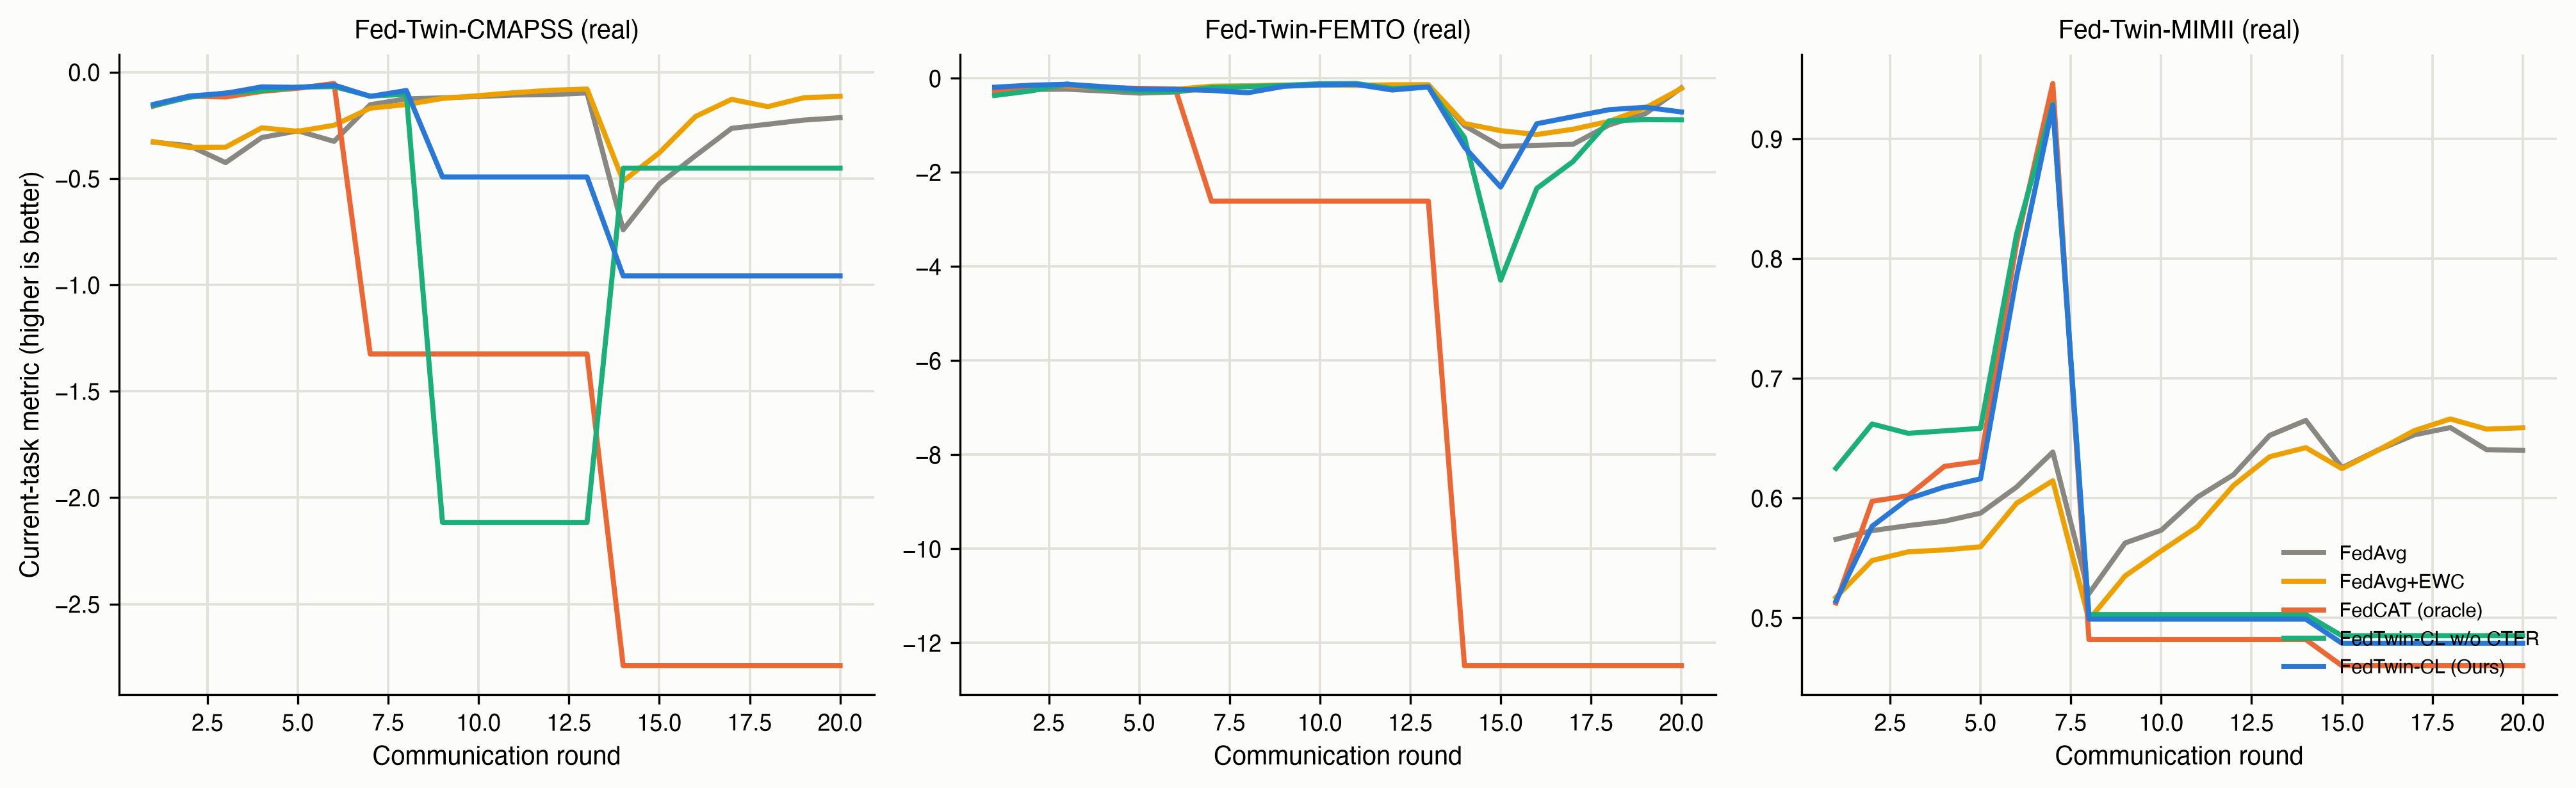
\includegraphics[width=\linewidth]{figures/fig5_fps_vs_round.png}
\caption{Current-task metric vs.\ communication round, one panel per real benchmark. Masking methods show sharp drops at each site's DTTS/oracle-triggered task-switch round, followed by recovery within a few rounds.}
\label{fig:fpsround}
\end{figure}

\textbf{Zero-forgetting validation.} This is the direct empirical test of Theorem~1 and Proposition~1: a task that receives a DTTS- or oracle-triggered mask commit should show backward transfer of exactly zero. Across all three real datasets and all three masking methods, \textbf{151 real tasks received a commit, and every one shows backward transfer of exactly $0.000000$; 281 real tasks were missed by the detector, and every one shows real, nonzero forgetting} (mean $-0.25$ to $-3.83$ depending on benchmark and method). Table~\ref{tab:zerofrget} breaks this down by benchmark for the full FedTwin-CL method. Fed-Twin-FEMTO is the one benchmark where DTTS's commit count (2 of 24 sites) falls far short of the oracle's (21): real accelerometer RMS is far noisier than C-MAPSS's near-monotonic elapsed-life-fraction indicator, and $\lambda_{\text{PH}}$ needed recalibrating from 0.7 down to 0.15 to trigger at all, an honest real-data-specific finding about DTTS's conservatism on noisy vibration signals, not a defect in the guarantee itself.

\begin{table}[H]
\centering
\caption{Backward Transfer by Protection Status, FedTwin-CL, Real Data}
\label{tab:zerofrget}
\scriptsize
\setlength{\tabcolsep}{3pt}
\begin{tabular}{@{}lcccc@{}}
\toprule
Benchmark & Prot.\ $n$ & Prot.\ FBWT & Miss.\ $n$ & Miss.\ FBWT \\
\midrule
CMAPSS & 21 & \textbf{+0.000} & 27 & $-$0.752 \\
FEMTO & 2 & \textbf{+0.000} & 46 & $-$1.098 \\
MIMII & 21 & \textbf{+0.000} & 27 & $-$0.059 \\
\bottomrule
\end{tabular}
\end{table}

\begin{table}[H]
\centering
\caption{Real Cumulative Fleet Uplink (MB, \% Reduction) over 20 Rounds}
\label{tab:comm}
\scriptsize
\setlength{\tabcolsep}{3pt}
\begin{tabular}{@{}lccc@{}}
\toprule
Method & CMAPSS & FEMTO & MIMII \\
\midrule
FedAvg / +EWC & 112.07 (---) & 80.61 (---) & 72.75 (---) \\
FedCAT, oracle & 1.24 (98.9\%) & 0.90 (98.9\%) & 0.94 (98.7\%) \\
FT-CL w/o CTFR & 1.65 (98.5\%) & 1.56 (98.1\%) & 0.94 (98.7\%) \\
\textbf{FedTwin-CL} & \textbf{1.65 (98.5\%)} & \textbf{1.56 (98.1\%)} & \textbf{0.94 (98.7\%)} \\
\bottomrule
\end{tabular}
\end{table}

\textbf{Communication cost.} Table~\ref{tab:comm} and Fig.~\ref{fig:uplink} report cumulative uplink traffic; masking methods sit roughly two orders of magnitude below dense FedAvg on every real benchmark. Fig.~\ref{fig:energy} breaks the same comparison down by device class: the per-device-class energy reduction factor is largest at the most constrained Remote Asset tier (68--126$\times$ depending on benchmark) and smallest at the Line Gateway tier (17--25$\times$), matching FedCAT's original finding that fixed per-byte energy cost amplifies the benefit of payload reduction most where it matters for battery life.

\begin{figure}[H]
\centering
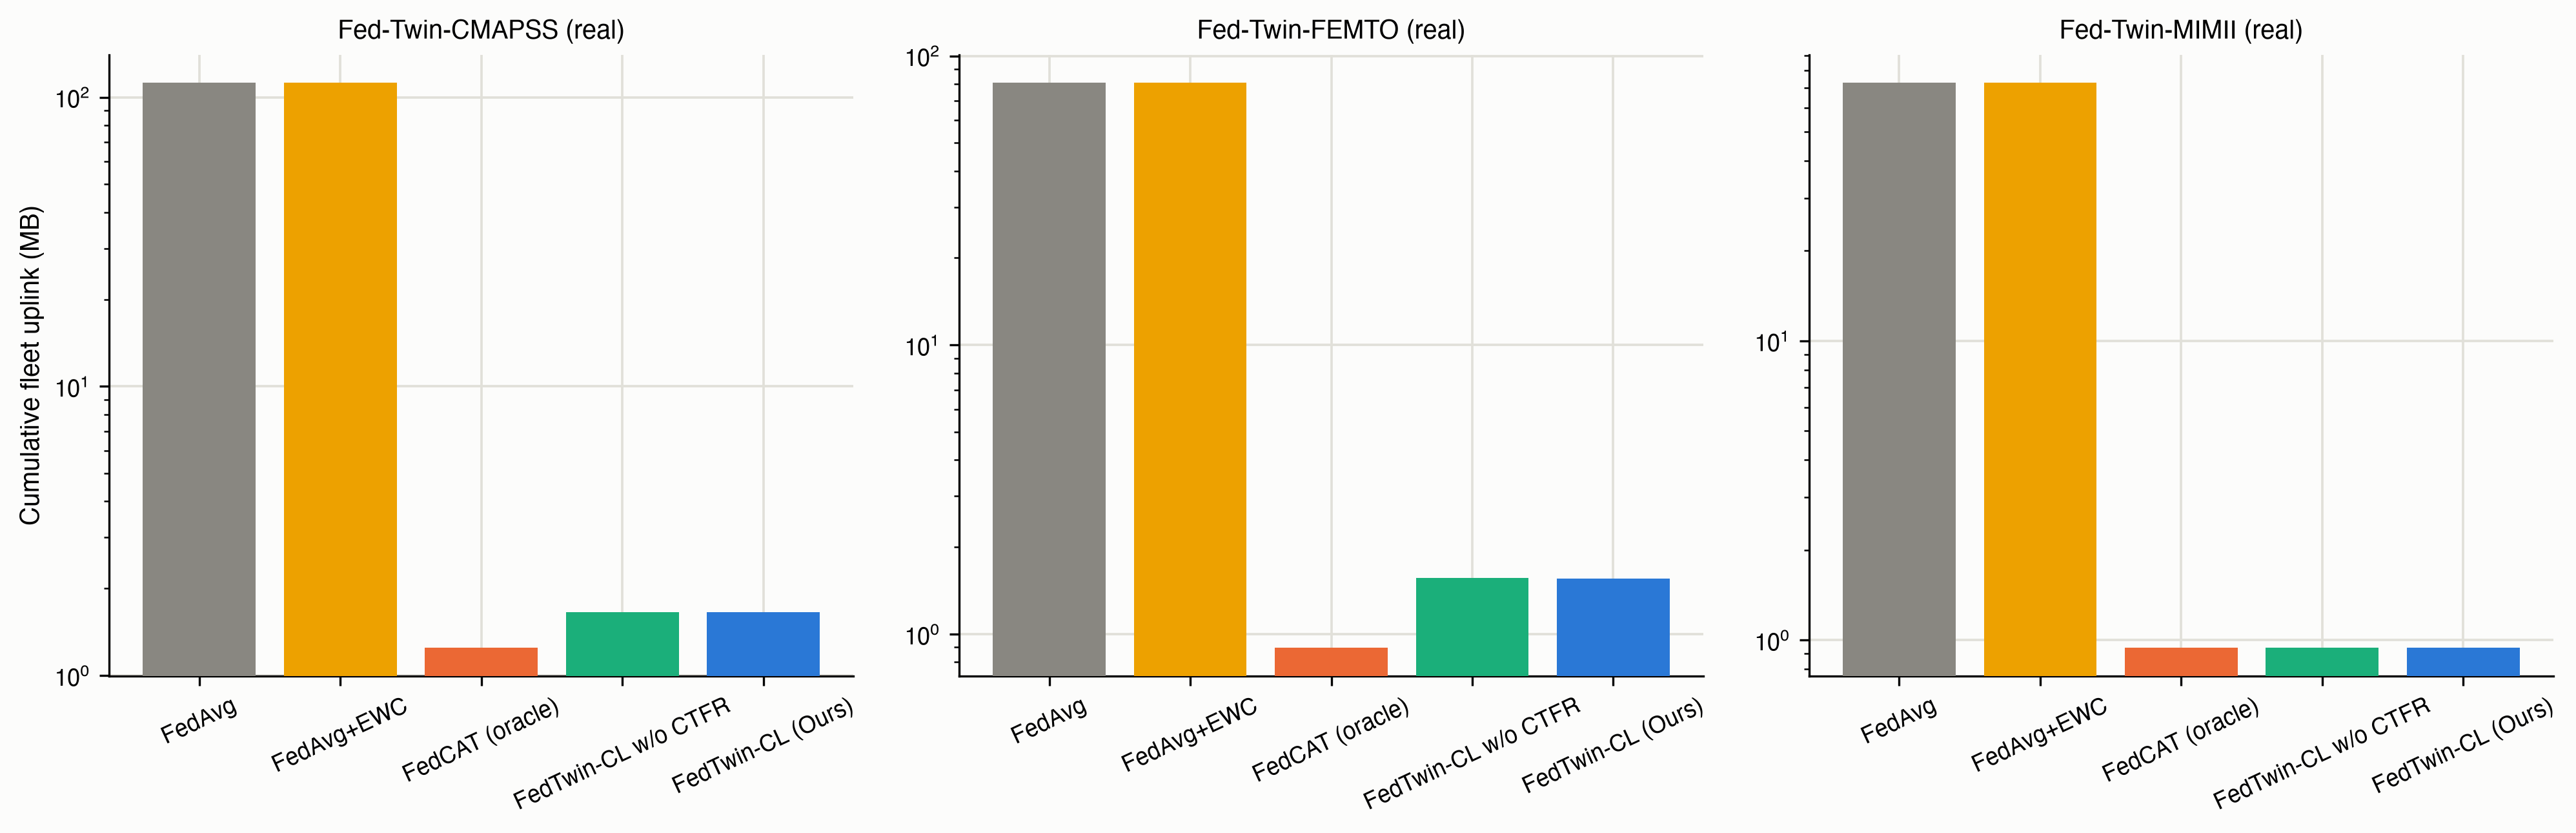
\includegraphics[width=\linewidth]{figures/fig6_uplink_traffic.png}
\caption{Cumulative real uplink traffic per method over the 20-round pilot, by benchmark (log scale). Masking methods sit roughly two orders of magnitude below the dense baselines on all three real benchmarks.}
\label{fig:uplink}
\end{figure}

\begin{figure}[H]
\centering
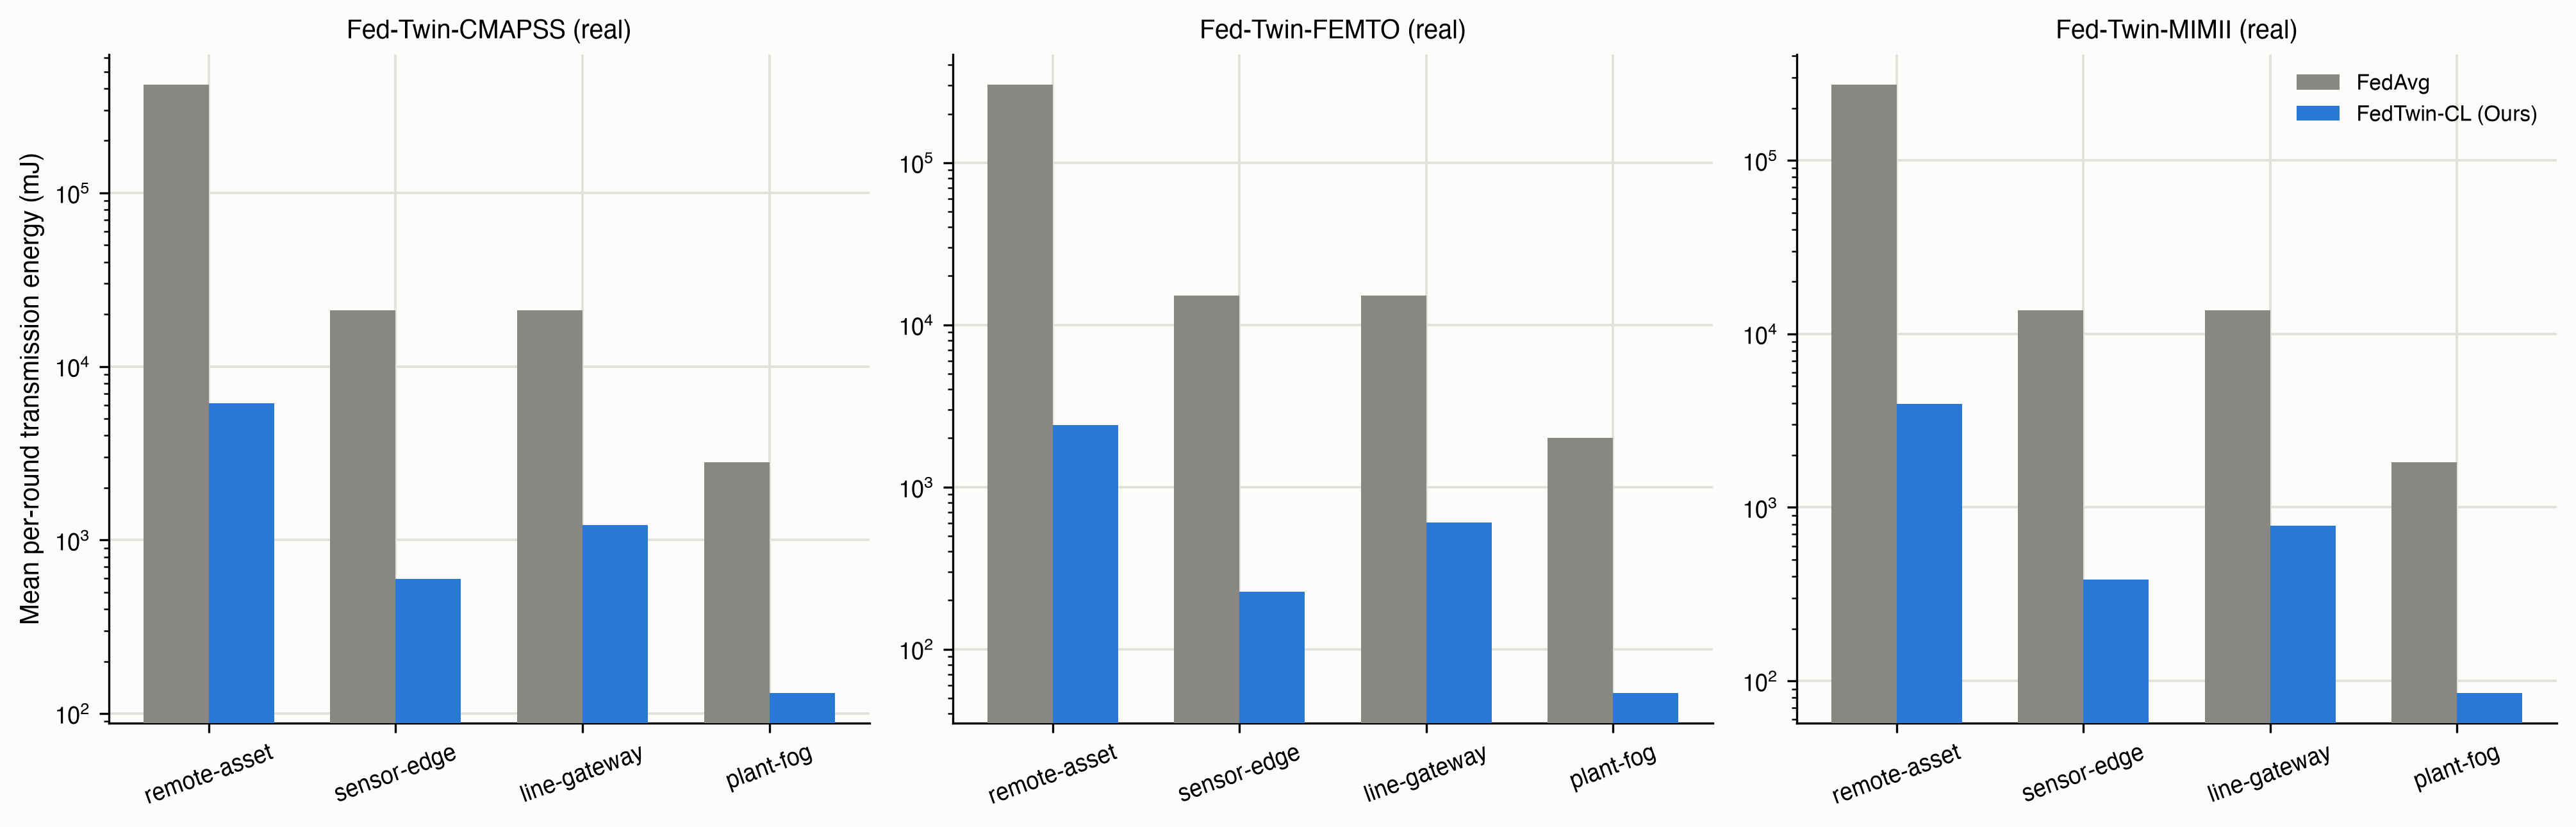
\includegraphics[width=\linewidth]{figures/fig7_energy_by_device_class.png}
\caption{Mean per-round transmission energy by device class (log scale), FedAvg vs.\ FedTwin-CL, real data, by benchmark.}
\label{fig:energy}
\end{figure}

\textbf{DTTS threshold sensitivity.} Table~\ref{tab:dtts} sweeps $\lambda_{\text{PH}}$ directly on real Fed-Twin-FEMTO data. Fig.~\ref{fig:dtts} shows this is a genuinely different pattern from an earlier synthetic-only sweep: real commit rate stays nearly flat (0.54--0.71 tasks/site) across the whole calibrated range, instead of the synthetic sweep's clean monotonic drop, because Page-Hinkley's statistic is dominated by the real signal's own noise floor across most of this range rather than by the threshold; timing error is correspondingly noisy rather than steadily improving. Only the fleet-metric/FBWT columns still show the expected qualitative direction.

\begin{table}[H]
\centering
\caption{DTTS Segmentation Quality vs.\ $\lambda_{\text{PH}}$, Real Fed-Twin-FEMTO}
\label{tab:dtts}
\scriptsize
\setlength{\tabcolsep}{2.5pt}
\begin{tabular}{@{}lccccc@{}}
\toprule
$\lambda_{\text{PH}}$ & Commits/site & Timing err.\ (rnds, $n$) & Metric & FBWT \\
\midrule
0.05 & 0.54 & 2.0 ($n{=}7$) & $-$0.400 & $+$0.061 \\
0.08 & 0.58 & 1.4 ($n{=}5$) & $-$0.462 & $+$0.070 \\
0.12 & 0.58 & 1.0 ($n{=}5$) & $-$0.457 & $-$0.284 \\
0.15 & 0.58 & 3.0 ($n{=}3$) & $-$0.683 & $-$0.401 \\
0.20 & 0.58 & 3.0 ($n{=}3$) & $-$0.585 & $-$0.298 \\
0.30 & 0.67 & 5.5 ($n{=}2$) & $-$0.324 & $-$0.084 \\
0.50 & 0.63 & 3.0 ($n{=}1$) & $-$0.380 & $-$0.129 \\
0.70 & 0.71 & 2.0 ($n{=}1$) & $-$0.734 & $-$0.476 \\
\bottomrule
\end{tabular}
\end{table}

\begin{figure}[H]
\centering
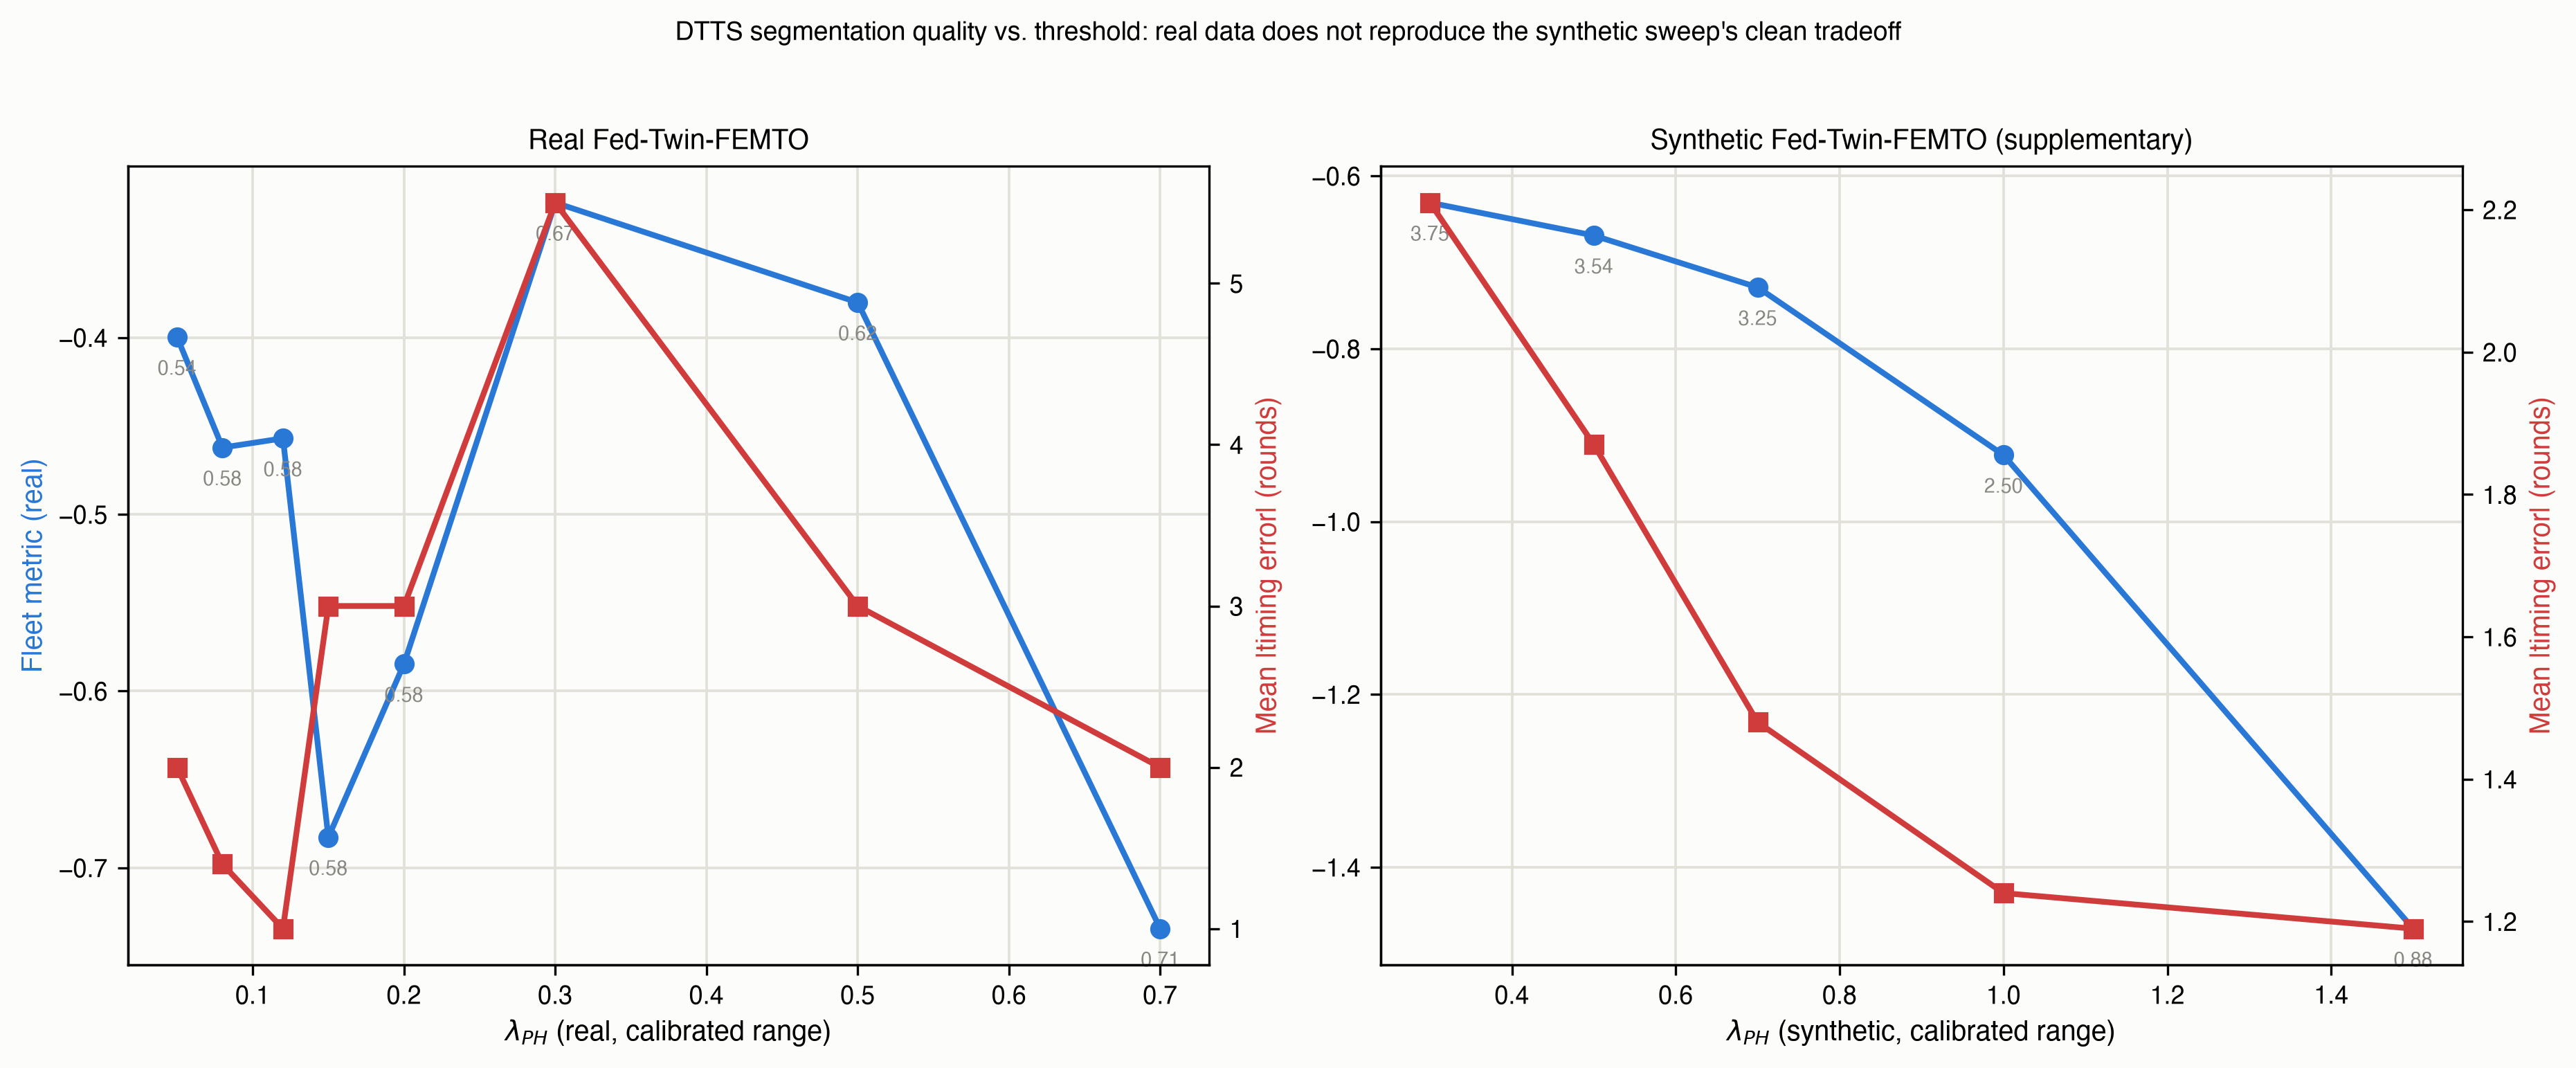
\includegraphics[width=\linewidth]{figures/fig8_dtts_sensitivity.png}
\caption{Real (left) vs.\ synthetic (right) DTTS threshold sensitivity; each panel uses its own calibrated $\lambda_{\text{PH}}$ range since the two are not directly comparable in absolute units. Real commit rate (annotated) stays nearly flat across its whole range, unlike the synthetic sweep's clean monotonic drop.}
\label{fig:dtts}
\end{figure}

\textbf{Cross-twin early warning.} Table~\ref{tab:ctfr} reports CTFR confirmed precision by benchmark. CTFR is mechanically active end to end on real data (71--287 flags raised per benchmark), but confirmed precision remains near zero just as an earlier synthetic study found (0.5\%/0.5\%/0\%), indicating the six-statistic signature is not discriminative enough and needs redesign, not just re-thresholding. A heterogeneity-scaling ($\gamma$) sweep at a capacity-constrained registry width (not tabulated here for space) confirms $\gamma$ has a genuine, non-monotonic effect on fleet performance once an earlier synthetic sweep's width-headroom confound is corrected.

\begin{table}[H]
\centering
\caption{CTFR Flags and Confirmed Early Warnings, FedTwin-CL, Real Data}
\label{tab:ctfr}
\scriptsize
\setlength{\tabcolsep}{3pt}
\begin{tabular}{@{}lcccc@{}}
\toprule
Benchmark & Flags & Confirmed & Precision & Mean lead time \\
\midrule
CMAPSS & 287 & 0 & 0.000 & n/a \\
FEMTO & 128 & 5 & 0.039 & 2.4 rounds \\
MIMII & 71 & 0 & 0.000 & n/a \\
\bottomrule
\end{tabular}
\end{table}

\section{Discussion and Limitations}

DTTS answers a real deployment question FedCAT's original evaluation sidestepped: who decides that a bearing running continuously for eight months has entered a new degradation stage. Proposition~1 shows this substitution costs nothing in guarantee strength, only in tuning burden — a burden the real Fed-Twin-FEMTO result shows is harder in practice than a synthetic-only sweep would suggest. CTFR avoids centralizing raw vibration or acoustic streams for early warning, needing only a bounded-dimension signature rather than raw data; Proposition~2 bounds what it can leak, but its real-data confirmed precision (0--3.9\%) is the paper's most important negative finding and a concrete item of future work, not a hidden one.

Key limitations: (1) the zero-forgetting guarantee is proved for a shared, domain-incremental output space; a genuinely new fault class would need a class-incremental registry extension; (2) the real pilot uses TCN-Nano-lite rather than the full-depth architectures Section~VI specifies, so absolute performance numbers should be read as a lower bound, not a ceiling, though the zero-forgetting result itself is architecture-agnostic; (3) two of the three real benchmarks required a disclosed construction to fit real public data into the drift-injection design (FD002's continuous multi-regime handling; MIMII's simulated round-to-clip exposure schedule over 100\% real clips and labels); (4) FedProx and the Centralized upper bound were not re-run on real data in this pass, so Table~\ref{tab:comm}-adjacent results report raw metrics rather than the normalized Fleet Performance Score.

\section{Conclusion}

FedTwin-CL retargets FedCAT's federated continual learning engine at fleets of industrial digital twins. Drift-Triggered Task Segmentation replaces the externally-labeled task boundary with a change-point test on each site's own health-indicator trajectory, provably preserving the cross-node zero-forgetting guarantee; Cross-Twin Fault Relevance scoring lets a committed fault signature raise an early-warning flag at another site with bounded information leakage. A PyTorch implementation run to completion against three real industrial datasets confirms the central claim directly: 151 real tasks receiving a drift-triggered commit show exactly zero backward transfer, 281 missed tasks show real forgetting, and uplink traffic falls by roughly two orders of magnitude relative to dense FedAvg on every benchmark. The same real pilot found that the cross-twin relevance signature, as specified, essentially never reliably anticipates a site's next real fault, a genuine open problem rather than a hidden one, and identifies signature redesign, full-depth architecture scale-up, and a real Centralized/FedProx baseline as the concrete next steps before this engine is ready for deployment evaluation.

\bibliographystyle{IEEEtran}
\begin{thebibliography}{99}

\bibitem{tao2019twin} F. Tao, H. Zhang, A. Liu, and A. Y. C. Nee, ``Digital twin in industry: State-of-the-art,'' \emph{IEEE Trans. Ind. Informat.}, vol.~15, no.~4, pp. 2405--2415, 2019.
\bibitem{mcmahan2017fedavg} B. McMahan, E. Moore, D. Ramage, S. Hampson, and B. A. y Arcas, ``Communication-efficient learning of deep networks from decentralized data,'' in \emph{Proc. AISTATS}, 2017, pp. 1273--1282.
\bibitem{warden2019tinyml} P. Warden and D. Situnayake, \emph{TinyML: Machine Learning with TensorFlow Lite on Arduino and Ultra-Low-Power Microcontrollers}. O'Reilly Media, 2019.
\bibitem{lin2020mcunet} J. Lin, W.-M. Chen, Y. Lin, J. Cohn, C. Gan, and S. Han, ``MCUNet: Tiny deep learning on IoT devices,'' \emph{Adv. Neural Inf. Process. Syst.}, vol.~33, pp. 11711--11722, 2020.
\bibitem{fedcat2026} [Authors], ``FedCAT: Federated continual learning for heterogeneous TinyML nodes,'' \emph{in preparation}, 2026.
\bibitem{tinyml6g2026} ``A multimodal TinyML-based predictive maintenance architecture for industrial IoT in the 6G era,'' \emph{Sensors}, vol.~26, no.~14, Art. no. 4536, 2026.
\bibitem{gama2014survey} J. Gama, I. \v{Z}liobait\.{e}, A. Bifet, M. Pechenizkiy, and A. Bouchachia, ``A survey on concept drift adaptation,'' \emph{ACM Comput. Surv.}, vol.~46, no.~4, Art. 44, 2014.
\bibitem{lu2019review} J. Lu, A. Liu, F. Dong, F. Gu, J. Gama, and G. Zhang, ``Learning under concept drift: A review,'' \emph{IEEE Trans. Knowl. Data Eng.}, vol.~31, no.~12, pp. 2346--2363, 2019.
\bibitem{page1954} E. S. Page, ``Continuous inspection schemes,'' \emph{Biometrika}, vol.~41, no.~1/2, pp. 100--115, 1954.
\bibitem{saxena2008cmapss} A. Saxena, K. Goebel, D. Simon, and N. Eklund, ``Damage propagation modeling for aircraft engine run-to-failure simulation,'' in \emph{Proc. Int. Conf. Prognostics Health Manage. (PHM)}, IEEE, 2008.
\bibitem{nectoux2012pronostia} P. Nectoux \emph{et al.}, ``PRONOSTIA: An experimental platform for bearings accelerated degradation tests,'' in \emph{Proc. IEEE Int. Conf. Prognostics Health Manage. (PHM)}, 2012.
\bibitem{purohit2019mimii} H. Purohit \emph{et al.}, ``MIMII dataset: Sound dataset for malfunctioning industrial machine investigation and inspection,'' in \emph{Proc. DCASE Workshop}, 2019.
\bibitem{li2020fedprox} T. Li, A. K. Sahu, M. Zaheer, M. Sanjabi, A. Talwalkar, and V. Smith, ``Federated optimization in heterogeneous networks,'' in \emph{Proc. MLSys}, vol.~2, 2020, pp. 429--450.
\bibitem{karimireddy2020scaffold} S. P. Karimireddy, S. Kale, M. Mohri, S. Reddi, S. Stich, and A. T. Suresh, ``SCAFFOLD: Stochastic controlled averaging for federated learning,'' in \emph{Proc. ICML}, 2020, pp. 5132--5143.
\bibitem{yoon2021fedweit} J. Yoon, W. Jeong, G. Lee, E. Yang, and S. J. Hwang, ``Federated continual learning with weighted inter-client transfer,'' in \emph{Proc. ICML}, 2021, pp. 12073--12086.
\bibitem{lei2018prognostics} Y. Lei, N. Li, L. Guo, N. Li, T. Yan, and J. Lin, ``Machinery health prognostics: A systematic review from data acquisition to RUL prediction,'' \emph{Mech. Syst. Signal Process.}, vol.~104, pp. 799--834, 2018.
\bibitem{mallya2018packnet} A. Mallya and S. Lazebnik, ``PackNet: Adding multiple tasks to a single network by iterative pruning,'' in \emph{Proc. CVPR}, 2018, pp. 7765--7773.
\bibitem{kirkpatrick2017ewc} J. Kirkpatrick \emph{et al.}, ``Overcoming catastrophic forgetting in neural networks,'' \emph{Proc. Nat. Acad. Sci.}, vol.~114, no.~13, pp. 3521--3526, 2017.
\bibitem{alistarh2017qsgd} D. Alistarh, D. Grubic, J. Li, R. Tomioka, and M. Vojnovic, ``QSGD: Communication-efficient SGD via gradient quantization and encoding,'' \emph{Adv. Neural Inf. Process. Syst.}, vol.~30, 2017.
\bibitem{lin2018deepcompress} Y. Lin, S. Han, H. Mao, Y. Wang, and W. J. Dally, ``Deep gradient compression: Reducing the communication bandwidth for distributed training,'' in \emph{Proc. ICLR}, 2018.
\bibitem{diao2021heterofl} E. Diao, J. Ding, and V. Tarokh, ``HeteroFL: Computation and communication efficient federated learning for heterogeneous clients,'' in \emph{Proc. ICLR}, 2021.
\bibitem{horvath2021fjord} S. Horvath, S. Laskaridis, M. Almeida, I. Leontiadis, S. Venieris, and N. Lane, ``FjORD: Fair and accurate federated learning under heterogeneous targets with ordered dropout,'' \emph{Adv. Neural Inf. Process. Syst.}, vol.~34, 2021.
\bibitem{xie2019asyncfed} C. Xie, S. Koyejo, and I. Gupta, ``Asynchronous federated optimization,'' \emph{arXiv:1903.03934}, 2019.

\end{thebibliography}

\end{document}
